\documentclass[12pt]{article}
\usepackage{times} 			% use Times New Roman font

\usepackage[margin=1in]{geometry}   % sets 1 inch margins on all sides
\usepackage[hidelinks]{hyperref}               % for URL formatting
\usepackage[pdftex]{graphicx}       % So includegraphics will work
\setlength{\parskip}{1em}           % skip 1em between paragraphs
\setlength{\parindent}{0pt}         % disable indentation for whole document
\usepackage{indentfirst}            % indent the first line of each paragraph
\usepackage{datetime}
\usepackage[small, bf]{caption}
\usepackage{listings}               % for code listings
\usepackage{xcolor}                 % for styling code
\usepackage{multirow}
\usepackage{subcaption}     % for subfigures

\usepackage[normalem]{ulem} % This package enables underlining

%\setlength\intextsep{1.69cm} 

%New colors defined below
\definecolor{backcolour}{RGB}{246, 246, 246}   % 0xF6, 0xF6, 0xF6
\definecolor{codegreen}{RGB}{16, 124, 2}       % 0x10, 0x7C, 0x02
\definecolor{codepurple}{RGB}{170, 0, 217}     % 0xAA, 0x00, 0xD9
\definecolor{codered}{RGB}{154, 0, 18}         % 0x9A, 0x00, 0x12

%Code listing style named "gcolabstyle" - matches Google Colab
\lstdefinestyle{gcolabstyle}{
  basicstyle=\ttfamily\small,
  backgroundcolor=\color{backcolour},   
  commentstyle=\itshape\color{codegreen},
  keywordstyle=\color{codepurple},
  stringstyle=\color{codered},
  numberstyle=\ttfamily\footnotesize\color{darkgray}, 
  breakatwhitespace=false,         
  breaklines=true,                 
  captionpos=b,                    
  keepspaces=true,                 
  numbers=left,                    
  numbersep=5pt,                  
  showspaces=false,                
  showstringspaces=false,
  showtabs=false,                  
  tabsize=2
}

\lstset{style=gcolabstyle}      %set gcolabstyle code listing

% to make long URIs break nicely
\makeatletter
\g@addto@macro{\UrlBreaks}{\UrlOrds}
\makeatother

% for fancy page headings
\usepackage{fancyhdr}
\setlength{\headheight}{13.6pt} % to remove fancyhdr warning
\pagestyle{fancy}
\fancyhf{}
\rhead{\small \thepage}
\chead{\small CS 532, Fall 2024} 
\lhead{\small HW\#4, Landers}  % EDIT THIS, REPLACE # with HW number

%-------------- Title ---------------%

\begin{document}

% EDIT THE ITEMS HERE
\begin{centering}
{\large\textbf{HW\#4 - Web Archiving, Part 2}}\\ 
Ethan Landers\\
Due: Sunday, October 27, 2024, by 11:59 PM\\
\end{centering}

%-------------- Q1 ---------------%

% The * after \section just says to not number the sections
\section*{Q1}

\emph{Q: What can you say about the relationship between the age of a URI-R and the number of its mementos?}

This question was challenging to answer because the URI-Rs I collected TimeMaps for had either 0 or 3 mementos each. I excluded the URI-Rs with 0 mementos from my analysis, resulting in plots for those with only 3 mementos. A scatter plot was not effective in this case due to the lack of variability in the number of mementos. Instead, I opted to create a box plot, which effectively illustrates the age of each memento across all the URI-Rs for which I grabbed TimeMaps.

\begin{figure}[h!]
    \centering
    % trim and clip are used to crop the image, trim=left bottom right top
    % width sets max width, height will be scaled appropriately
    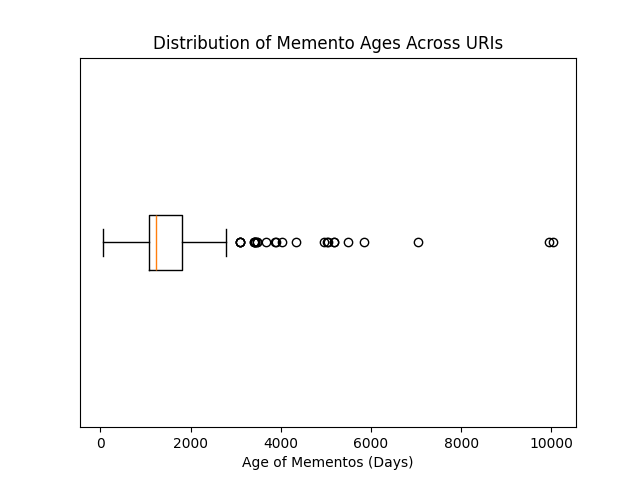
\includegraphics[trim=0 0 0 25, clip, width=\textwidth] {boxplot.png}
    \caption{Distribution of Mementos Ages Across URIs}
    \label{fig:boxplot}
\end{figure}

The results indicate that the majority of mementos for archived URI-Rs are between 1,000 and 2,000 days old, with a few outliers exceeding 2,000 days.

\emph{Q: What URI-R had the oldest memento? Did that surprise you?}

The URI-R that has the oldest memento from the URI-Rs that were analyzed was https://www.unc.edu, with the earliest memento date being 1997-04-27 05:36:51. I'm not that surprised by the result as the University of North Carolina Chapel Hill is a prestigious state university that is known for conducting research.

\emph{Q: How many URI-Rs had an age of $< 1$ week, meaning that their first memento was captured the same week you collected the data?}

It was concluded that zero URI-Rs had an age of less than 1 week after analysis. All the URI-Rs that I looked at had mementos that were captured more than a week ago (as of 10/26/2024).

%-------------- Q2 ---------------%

\section*{Q2}

\href{https://conifer.rhizome.org/ethan746/hw4-cs532}{\uline{Click here}} to access my Conifer public collection for Q2 of this assignment.

Figure \ref{fig:replay} shows the list of archived pages as well as the browser address bar after uploading the WARC file (created by archiving 10 webpages using Conifer) to ReplayWeb.page (\url{https://replayweb.page/}).

\begin{figure}[h!]
    \centering
    % trim and clip are used to crop the image, trim=left bottom right top
    % width sets max width, height will be scaled appropriately
    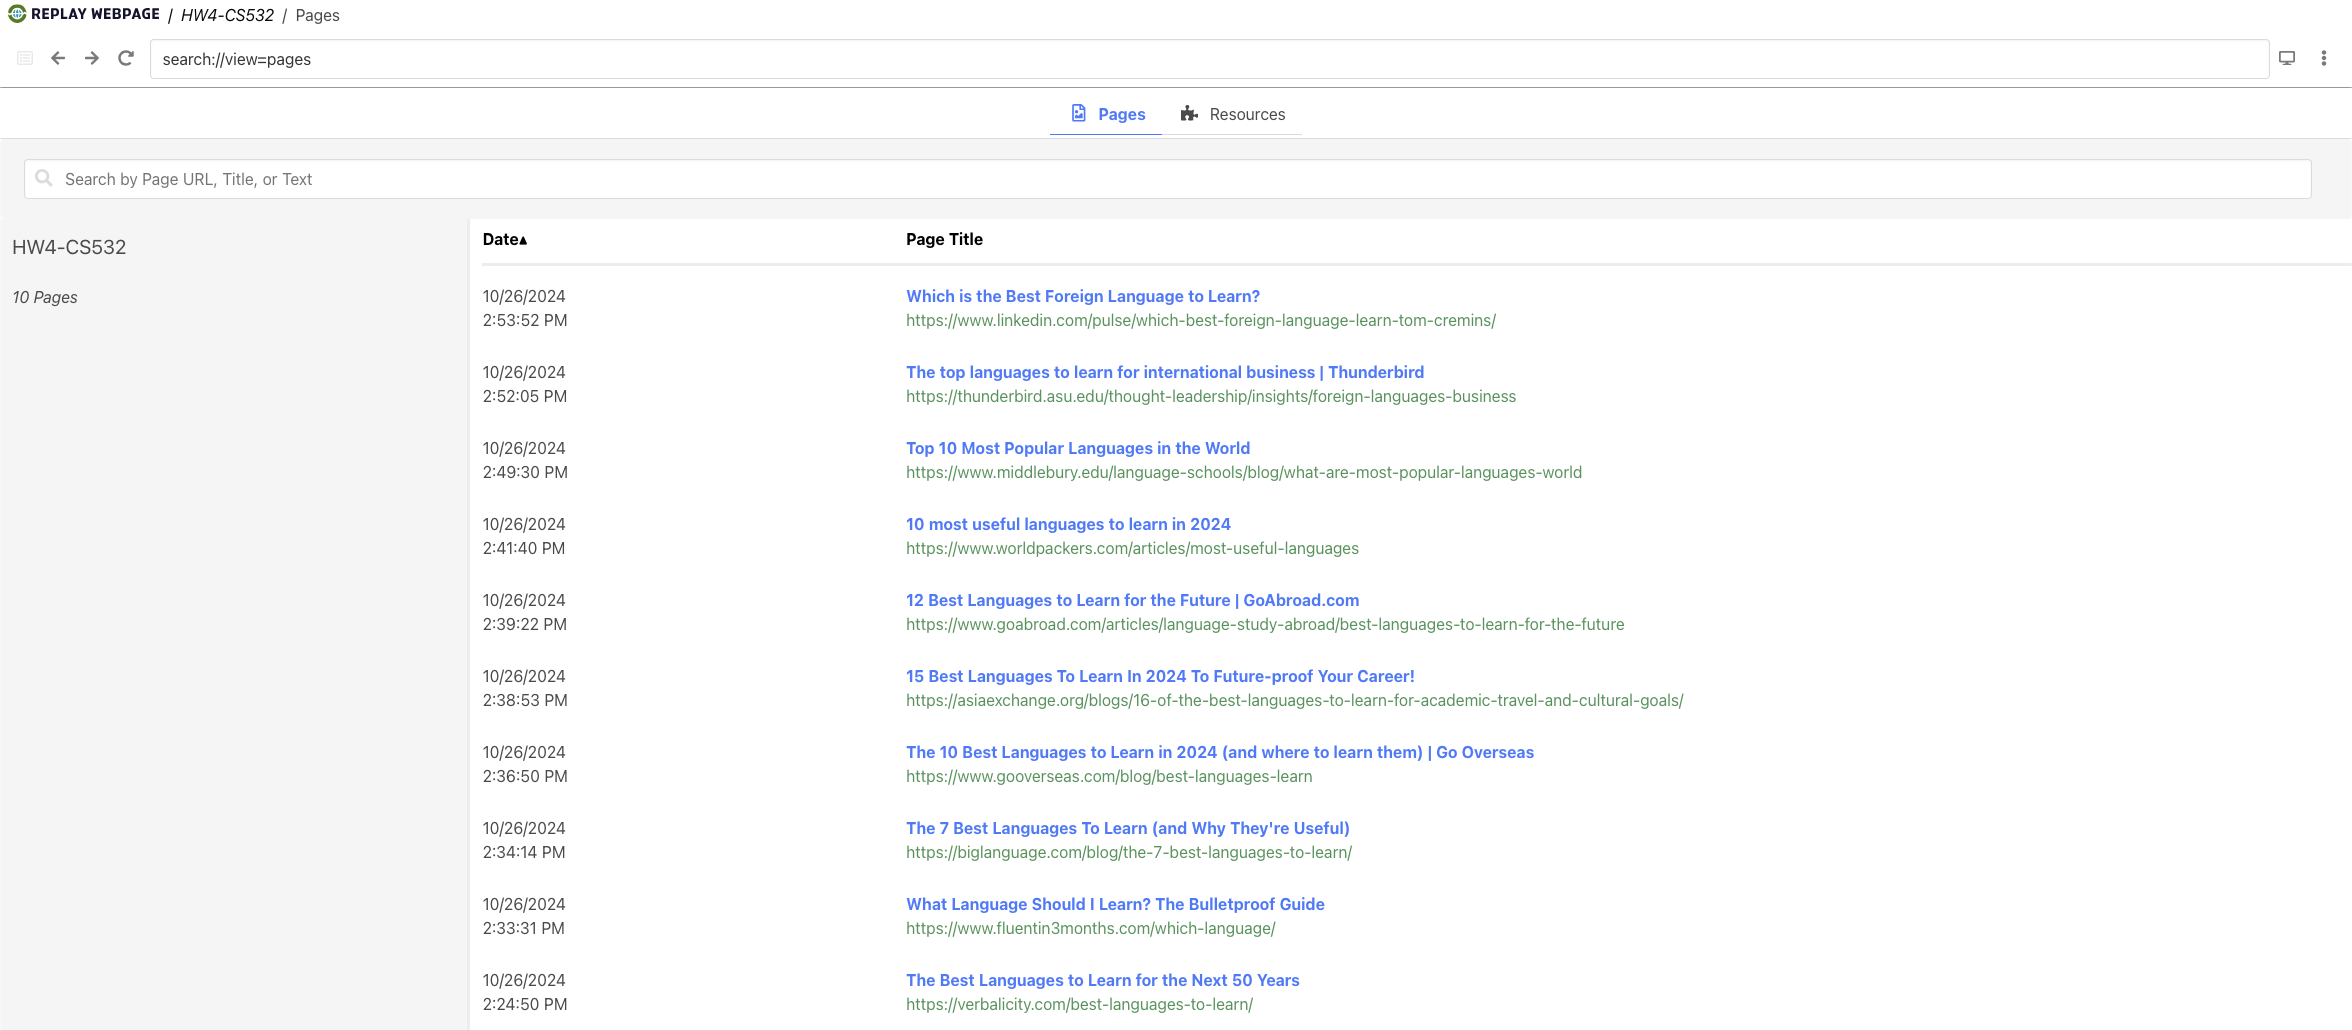
\includegraphics[trim=0 0 0 0, clip, width=\textwidth] {replay.png}
    \caption{ReplayWeb.page WARC file "Pages" Tab}
    \label{fig:replay}
\end{figure}

\emph{Q: Why did you choose this particular topic?}

I am a big language fan, and I speak Spanish self-taught. I want to learn a new language, but I have the hardest time choosing the next language to learn. Therefore, I chose to archive websites discussing the best foreign languages to learn. 

\emph{Q: Did you have any issues in archiving the webpages?}

For some websites, when I started the archiving process, a 404 error message would appear, and I couldn't archive the website that I wanted to. Otherwise, no issues. While capturing, I would scroll to the bottom of every webpage so the whole page could be captured.

\emph{Q: Do the archived webpages look like the original webpages?}

For the most part, the archived webpages look quite similar to their original webpages. Sometimes there is a minor formatting difference, but nonetheless very similar.

\emph{Q: How many URLs were archived in the WARC file? How does this compare to the number of Pages?}

A total of 1,140 URLs were archived in the WARC file, corresponding to 10 webpages. This indicates that each archived webpage contained a diverse array of resources, including images, scripts, and other types of content.

\begin{figure}[h!]
    \centering
    % trim and clip are used to crop the image, trim=left bottom right top
    % width sets max width, height will be scaled appropriately
    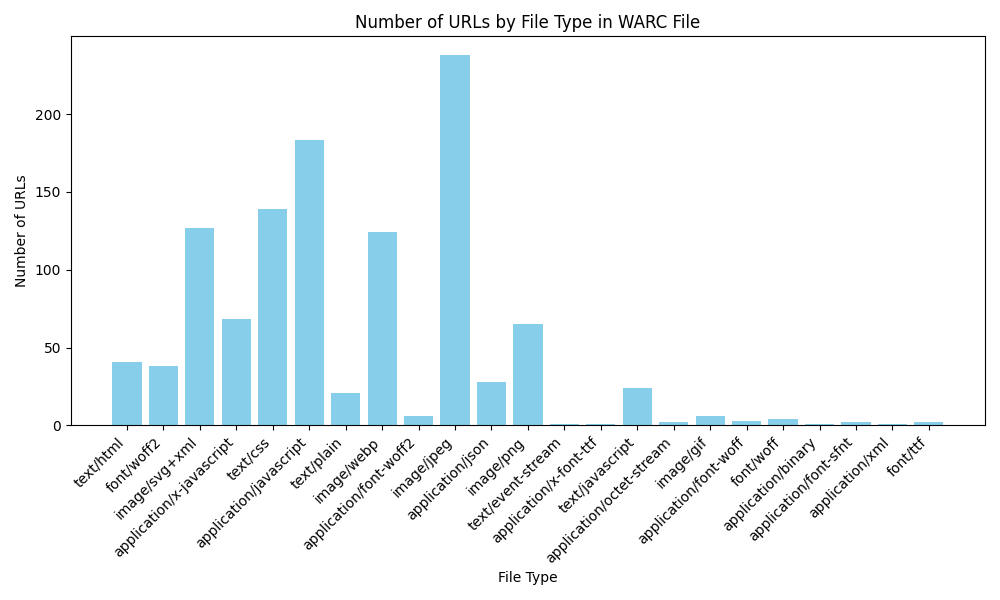
\includegraphics[trim=0 0 0 0, clip, width=\textwidth] {Q2.png}
    \caption{Number of URLs by File Type in WARC File}
    \label{fig:q2}
\end{figure}

\emph{Q: Which file type had the most URLs? Were you surprised by this?}

JPEG was the file type that had the most URLs. This doesn't surprise me as many web pages contain several JPEG image files.

%-------------- References ---------------%

\section*{References}

\begin{itemize}
    \item {Counters in Python, \url{https://www.geeksforgeeks.org/counters-in-python-set-1/}}
    \item{Python | datetime.timedelta() function, \url{https://www.geeksforgeeks.org/python-datetime-timedelta-function/}}
    \item {Warcio, \url{https://github.com/webrecorder/warcio}}
\end{itemize}

\end{document}

